\section{Релевантные работы}
\subsection{Введение}
%Базы знаний, декомпозиция, ЛВВ, рисунки, графики неточные вероятности, БСД.


\subsection{Обзор темы исследования}
 Теория вероятностных графических моделей~(ВГМ) являются одной из областей искусственного интеллекта, дающей возможность связать понятия данных, вероятностной логики и теории графов. Соединяя эти понятия исследователь получает возможность анализировать данные, принимая во внимание их связанность между собой (например последовательность состояний или причинно-следственные связи). К ВГМ относятся такие модели как марковские цепи и байесовские сети доверия, которые являются родственными алгебраическим байесовским сетям, являющимися объектом исследования данной работы. Вероятностные графические модели имеют широкое применение в ряде областей и давно подтвердили свою состоятельность, однако АБС выделяются среди прочих ВГМ за счет нескольких факторов. Одним из таких факторов  является структура АБС, предполагающая декомпозицию базы знаний на небольшие объемы тесно связанных между собой данных, что позволяет ускорить алгоритмы обработки за счет возможности работы с ограниченным набором элементов. 
 

 
Алгебраические байесовские сети представляются ненаправленными графами с идеалами конъюнктов в узлах. Конъюнктам приписывается либо скалярная~(точечная), либо интервальная оценка вероятности истинности. Назовем идеал конъюнктов с приписанными его элементам оценками вероятности истинности фрагментом знаний~(ФЗ). Фрагмент знаний строится над некоторым множеством атомов. Например для алфавита $A = \{x_1,x_2,x_3\}$  фрагмент знаний будет выглядеть, как на рисунке \ref{KP_3}. 

\begin{figure}[h!]
  \begin{center}
    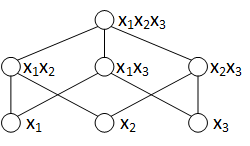
\includegraphics[width=.5\linewidth]{Conj_3_KP.png}
    \caption{Фрагмент знаний, построенный над тремя атомами.}
    \label{KP_3}
  \end{center}
\end{figure}


%Переделать АБС на с большим количеством ФЗ
На рисунке \ref{ABN} изображена алгебраическая байесовская сеть, состоящая из двух фрагментов знаний.

\begin{figure}[h!]
  \begin{center}
    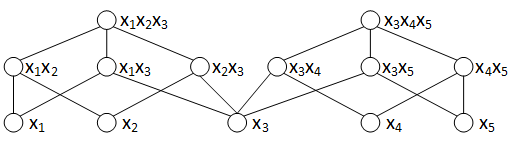
\includegraphics[width=.9\linewidth]{ABN_2.png}
    \caption{АБС, состоящая из двух фрагментов знаний.}
    \label{ABN}
  \end{center}
\end{figure}
    
Основным аппаратом для обработки существующих и получения новых знаний является логико-вероятностный вывод~(ЛВВ)~\cite{nsmv}. По уровню действия на сеть логико-вероятностный вывод делится на глобальный и локальный. ``Глобальный'' говорит нам о том, что в область нашего рассмотрения попадает вся сеть и входящие в нее ФЗ, а ``локальный'' о том, что область рассмотрения сужается до одного фрагмента знаний. Задачи, рассматриваемые в ЛВВ, включают в себя проверку непротиворечивости, поддержание непротиворечивости (для случая интервальных оценок), задачу априорного вывода и две задачи апостериорного вывода. 
    
В глобальном случае при проверке и поддержке непротиворечивости в сети, оценки вероятности истинности элементов сети проверяются на согласованность и, при возможности, уточняются. В локальном случае мы рассматриваем и работаем только с одним зафиксированным ФЗ из сети и проверяем на согласованность и пытаемся уточнить оценки только в нем, не затрагивая при этом остальные ФЗ сети. 
    
Априорный вывод~\cite{tul} заключается в том, что мы оцениваем вероятность истинности пропозициональной формулы, построенной над каким-то фиксированным алфавитом. В локальном виде вывода формула строится над тем же алфавитом, что и рассматриваемый ФЗ.
    
Задачи апостериорного вывода возникают тогда, когда в нашу сеть поступает новая обуславливающая информация, которую мы будем называть свидетельством. В глобальном случае свидетельство поступает во всю сеть и строится над алфавитом сети, а в локальном -- в выбранный ФЗ и строится над его алфавитом. Первая задача апостериорного вывода сводится к вычислению вероятности свидетельства на основе оценок вероятности истинности, заданных во фрагменте знаний. Вторая задача состоит в вычислении условных оценок вероятности истинности во фрагменте знаний с учетом поступившего свидетельства. В рамках теории алгебраических байесовских сетей разделяют три вида свидетельств: детерминированное, стохастическое и неточное. Детерминированное свидетельство является базовым и наиболее простым и операции с более сложными видами свидетельств так или иначе сводятся к детерминированному случаю. В глобальных операциях над сетью используются локальные операции, то есть обработка конкретных фиксированных ФЗ. Поэтому так важно изучение и развитие именно локального вывода и, в частности, апостериорного вывода с использованием детерминированного свидетельства, который будет рассмотрен в данной работе. 
    
Анализ чувствительности является одним из критериев оценки математической модели~\cite{WOS5_sensitivity,WOS2_sensitivity,WOS6_sensitivity}. Характеризуя степень колебания результата в зависимости от изменения входных данных, чувствительность имеет практическое предназначение и позволяют определить степень претенциозности к точности входных данных, что сказывается на количестве входных данных необходимых на вход соответствующему алгоритму для получения результата заданной точности.    

%ссылки из СЕЙМ и ИИТИ17

\subsection{Выводы по главе}


